\documentclass[20pt,margin=1in,innermargin=0in,blockverticalspace=-0.3in]{tikzposter}
\geometry{paperwidth=80cm,paperheight=120cm}
\usepackage[utf8]{inputenc}
\usepackage{amsmath}
\usepackage{amsfonts}
\usepackage{amsthm}
\usepackage{amssymb}
\usepackage{mathrsfs}
\usepackage{graphicx}
\usepackage{adjustbox}
\usepackage{enumitem}
\usepackage{booktabs}
\usepackage{array}
\usepackage{caption}
\captionsetup[figure]{
  skip=0pt % Adjust the space according to your needs
}
\usepackage[backend=biber,style=numeric,sorting=none]{biblatex}
\usepackage{emory-theme}

\usepackage{mwe} % for placeholder images

\addbibresource{refs.bib}
\renewcommand{\familydefault}{\sfdefault}
\renewcommand*{\bibfont}{\fontsize{17}{12}\selectfont}


% set theme parameters
\tikzposterlatexaffectionproofoff
\usetheme{EmoryTheme}
\usecolorstyle{EmoryStyle}

\title{Neural Network Reveals Gravitational Coupling of Endemic Measles Dynamics}
\author{Wyatt G.\relax ~Madden\textsuperscript{$\dagger$}, Jessica E.\relax ~Metcalf\textsuperscript{$\ddagger$}, Bryan T.\relax ~Grenfell\textsuperscript{$\ddagger$}, Max S.\relax Y.\relax ~Lau\textsuperscript{$\dagger$}}
\institute{\textsuperscript{$\dagger$}Department of Biostatistics \& Bioinformatics, Emory University,\\
\textsuperscript{$\ddagger$}Princeton University, NJ, USA\\}

\begin{document}
\maketitle
\centering
\begin{columns}
    \column{0.5}
    \block{Introduction}{
        \begin{minipage}{0.5\linewidth}
        Measles is an important infectious disease system, both for its immediate relevance to public health and for the study of non-linear spatio-temporal disease dynamics. 
        Traditional mechanistic models are often unable to fully capture the complicated nonlinear spatio-temporal dynamics inherent in measles transmission. 
        Here we develop a high-dimensional neural-network-based model to forecast endemic measles outbreaks, with the aim of providing both prediction accuracy and interpretability and inference of mechanistic drivers.
  \end{minipage}%
  \hfill
  \begin{minipage}{0.5\linewidth}
        \begin{tikzfigure}[Map of England and Wales, with cities/towns colored by log measles cases on first biweek of 1961.]
            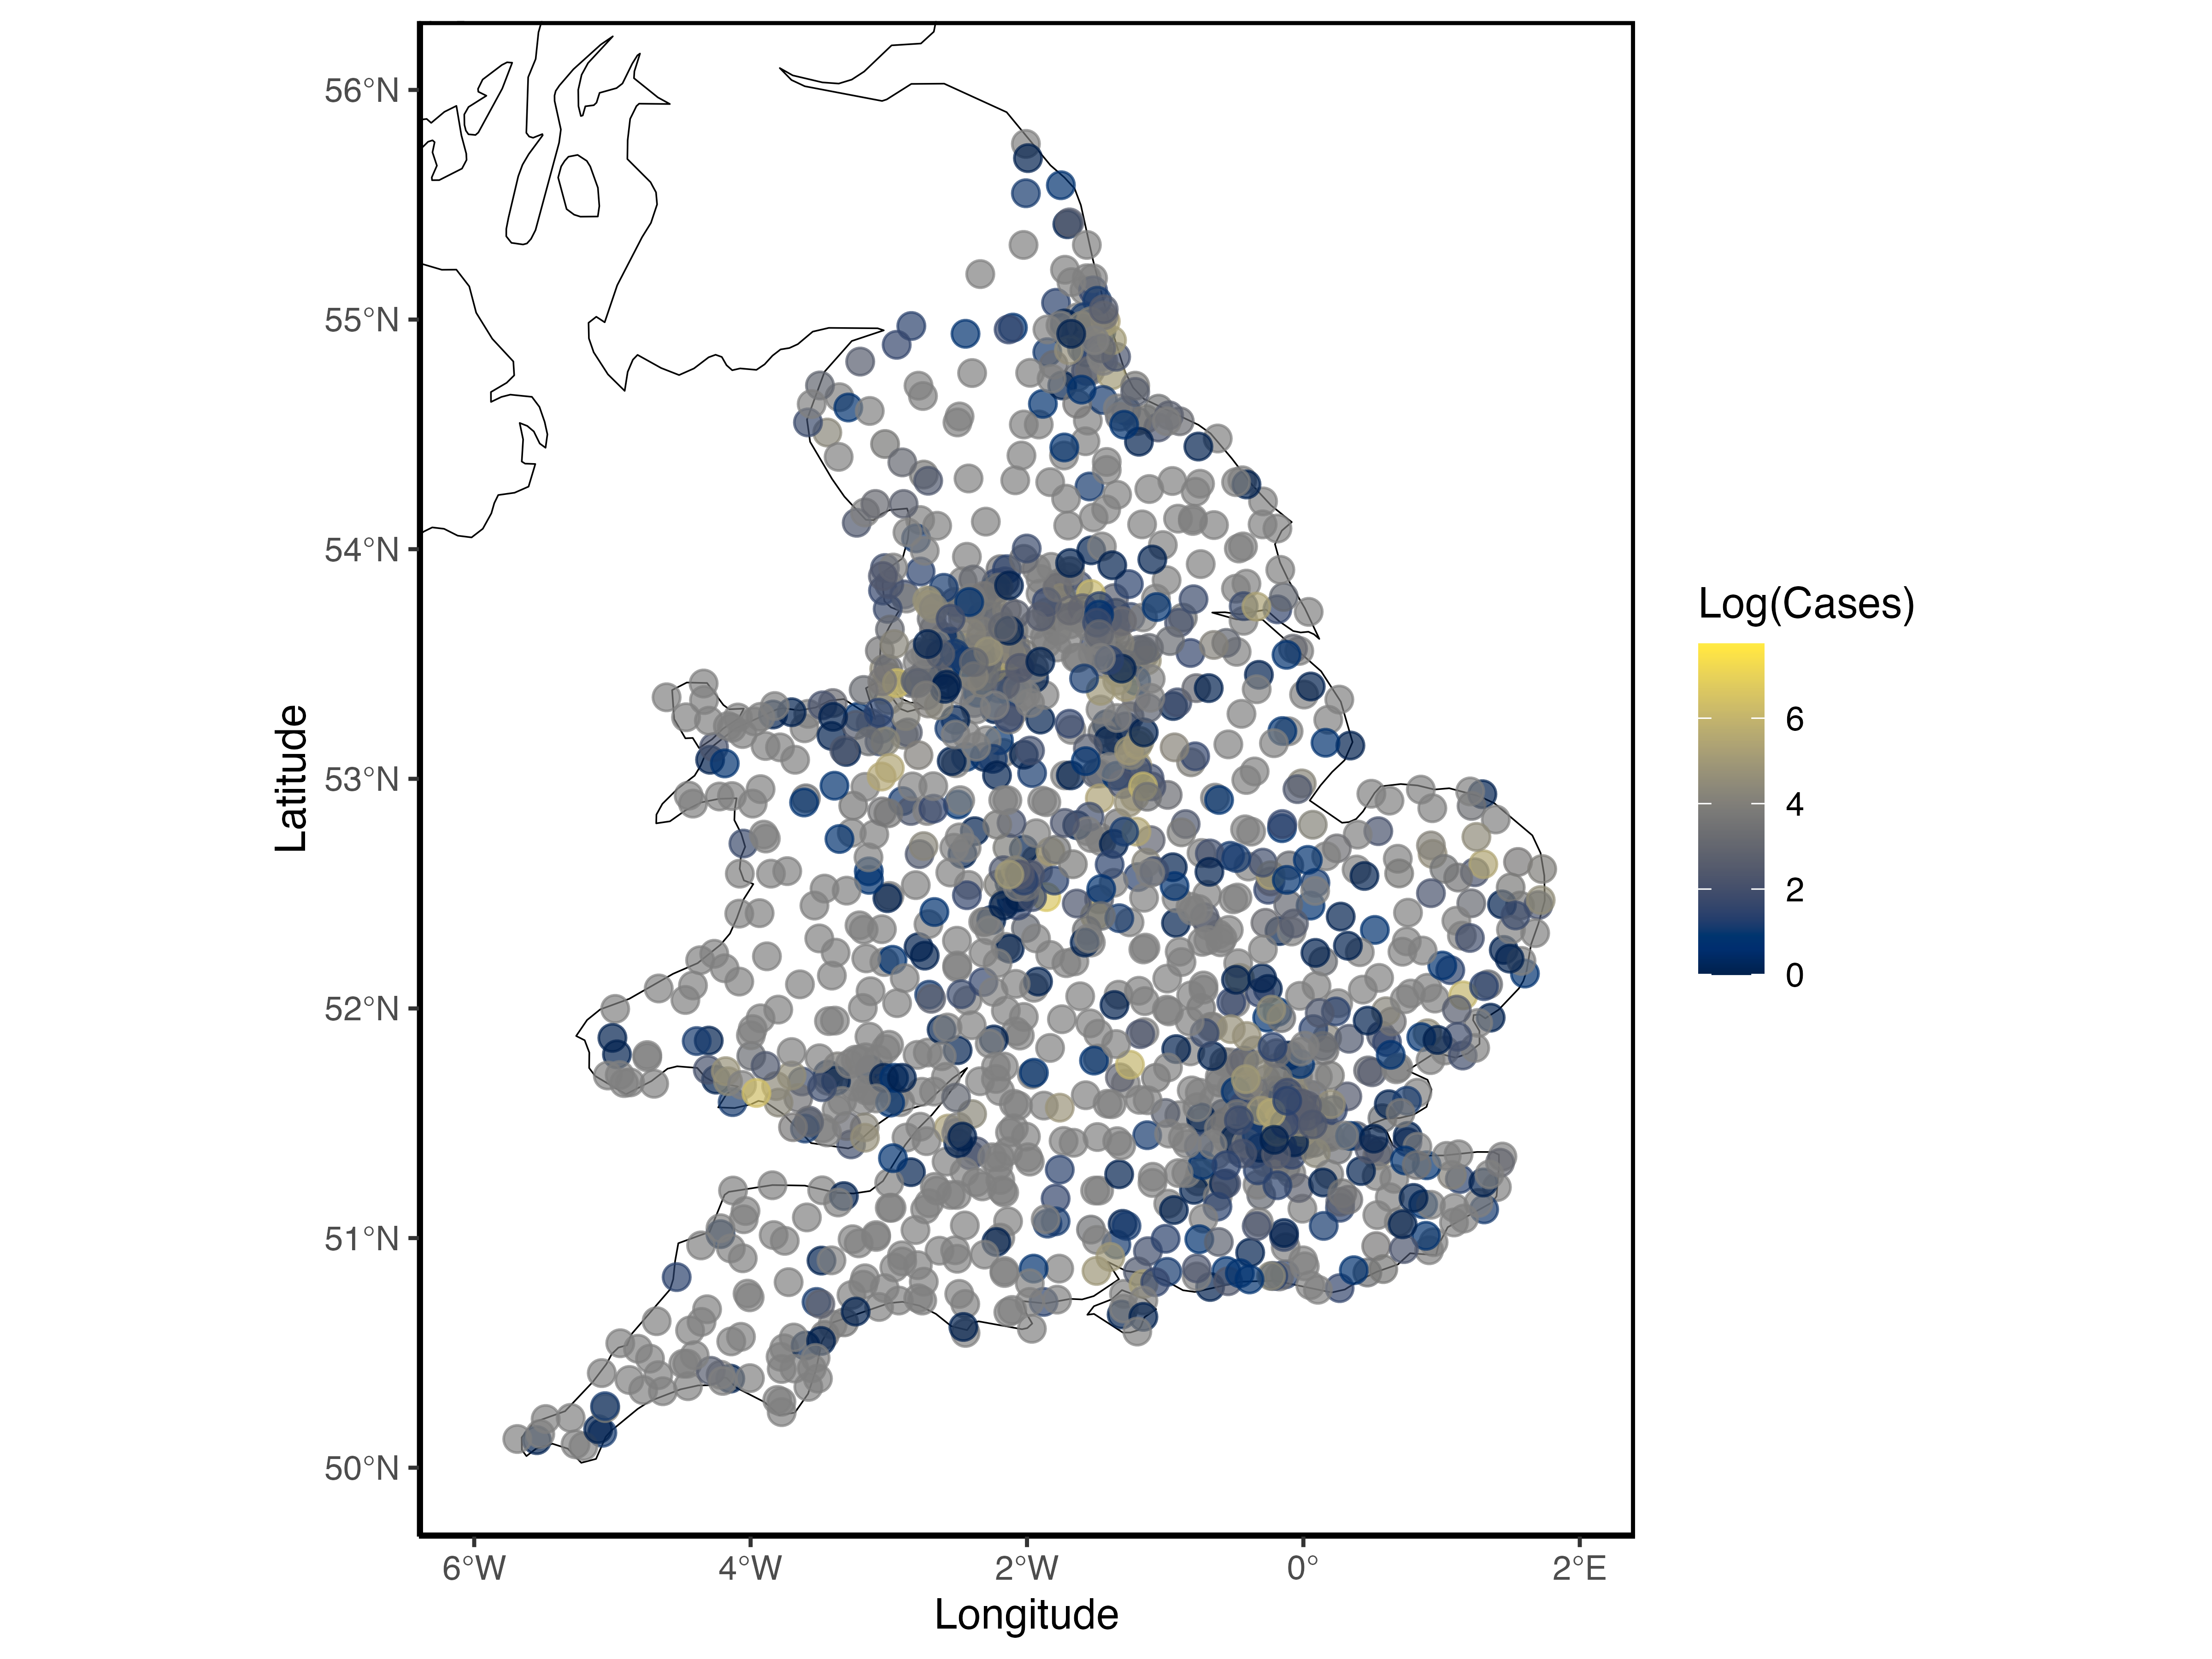
\includegraphics[width=0.9\linewidth]{figures/england_wales_map.png}
            \vspace{-0.5em}
            \label{fig:ewmap}
        \end{tikzfigure}
            \vspace{1em}
  \end{minipage}

        We demonstrate forecast accuracy for high and low population cities/towns for time steps ahead ranging from 1 to 52 biweeks, and employ feature importance methods to demonstrate the learning of coupled gravity dynamics. 

        \vspace{2em}
    }

    \block{Data \& Methods}{

        \begin{minipage}{0.6\linewidth}
        \begin{tikzfigure}[Feed-forward neural network architecture.]
            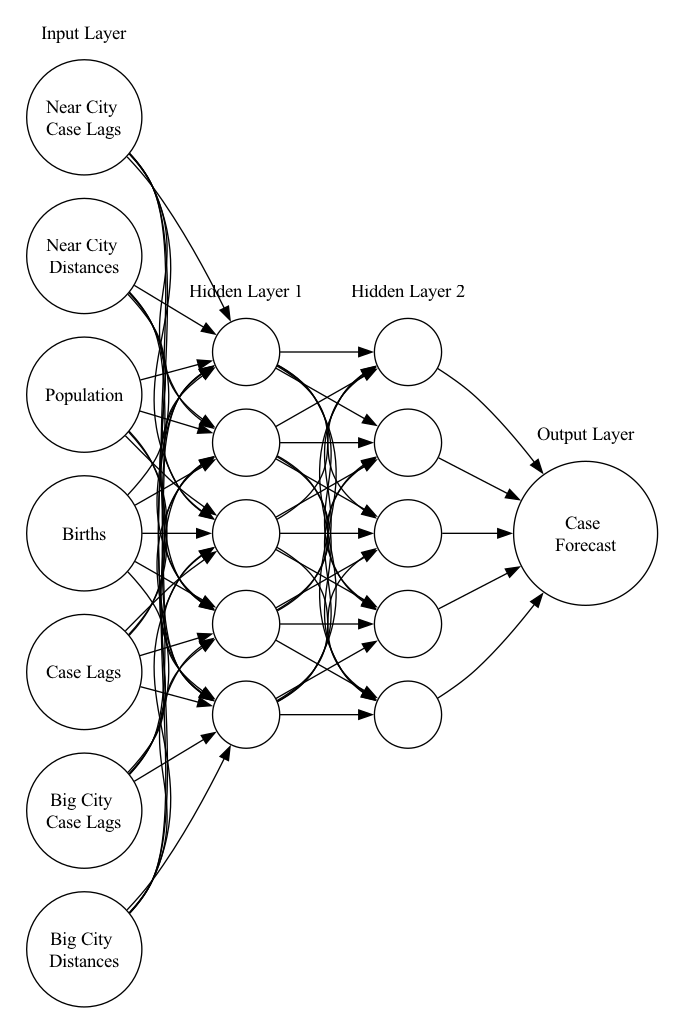
\includegraphics[width=0.4\linewidth]{figures/feedforward_network_structure.png}
            \vspace{-0.5em}
            \label{fig:nn_arch}
        \end{tikzfigure}
            \vspace{1em}
        \end{minipage}%
  \hfill
  \begin{minipage}{0.4\linewidth}
        Our data consists of biweekly measles case counts across 1,452 cities/towns in the United Kingdom during the pre-vaccination period from 1951 to 1964. 
        The forecast goal was to predict k-step ahead case counts for all cities/towns, for $k \in \{1, 2, \dots, 52\}$ using a range of features. 
        For each $k$-step ahead we fit a separate feed-forward neural network with 2 hidden layers of dimension 962, linear input/output layers, and ReLu activation functions (Figure~\ref{fig:nn_arch}).
  \end{minipage}

        Features include lagged case counts, high population city lagged case counts and distances (defined as a population greater than 300k, of which there are seven), nearest ten city lagged case counts and distances, births, population. 
        Lagged features range from $t - k$ to $t - 130$, where $t$ is the target time step. 
        Birth and population features are from the nearest time step less than or equal to $t - k$ while still sharing the same biweek of the year. 
        Neural networks are fit using the Adam optimizer with MSE loss, and are trained on 70\% of the data (cases ranging from 1951 to 1960), with 30\% of the data (cases ranging from 1960 to 1964) held out for testing.

        We compare the neural networks to TSIR (time-series susceptible-infected-recovered) models, a popular semi-mechanistic technique that has been shown to handle the dynamics of measles outbreaks well \cite{finkenstadt2000time}.
        TSIR provides a computationally inexpensive and highly tractable alternative to the classic SIR compartmental model, and is described by the following equations:
        \[
            E[I_{t+1}] = \beta_{t + 1} I_t^\alpha S_t \quad \quad
            S_{t+1} = B_{t + 1} + S_t - I_{t+1} \\
        \]
        \vspace{1em}
    }
    \block{Performance}{
        The neural network generally performed better than TSIR for all $k$-steps ahead, across different population sizes. 
        While the neural network performed well for long forecasts in high-population cities (Figure~\ref{fig:preds}), the level of improvement is most pronounced for small $k$-steps ahead in low population cities/towns that have sporadic and brief outbreaks (Figures~\ref{fig:rmse},\ref{fig:cor}).

        \begin{tikzfigure}[52-step ahead test set neural network forecasts, TSIR forecasts, and true case values for London and Manchester]
            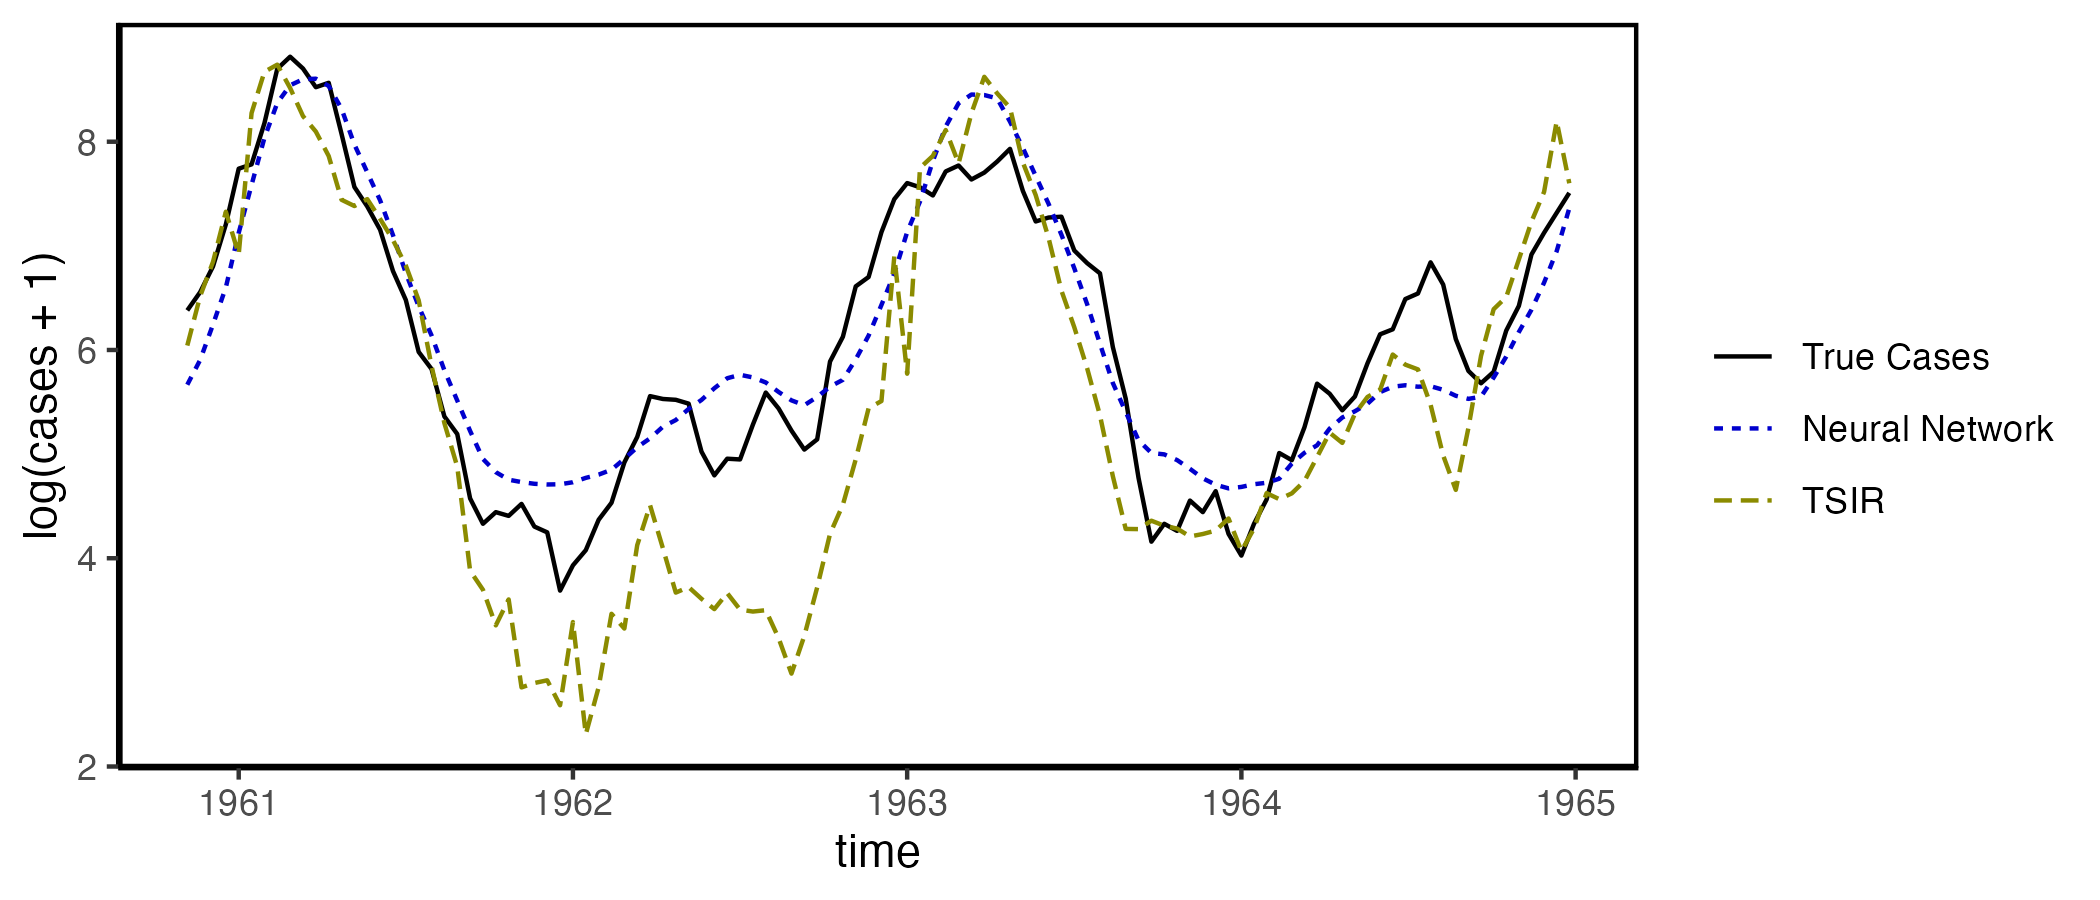
\includegraphics[width=0.8\linewidth]{figures/man_lond_logged_k52.png}
            \vspace{-1em}
             \label{fig:preds}
        \end{tikzfigure}

        \begin{tikzfigure}[Within-city neural network RMSE over TSIR RMSE, colored by log(population), facetted by $k$-step ahead forecast.]
            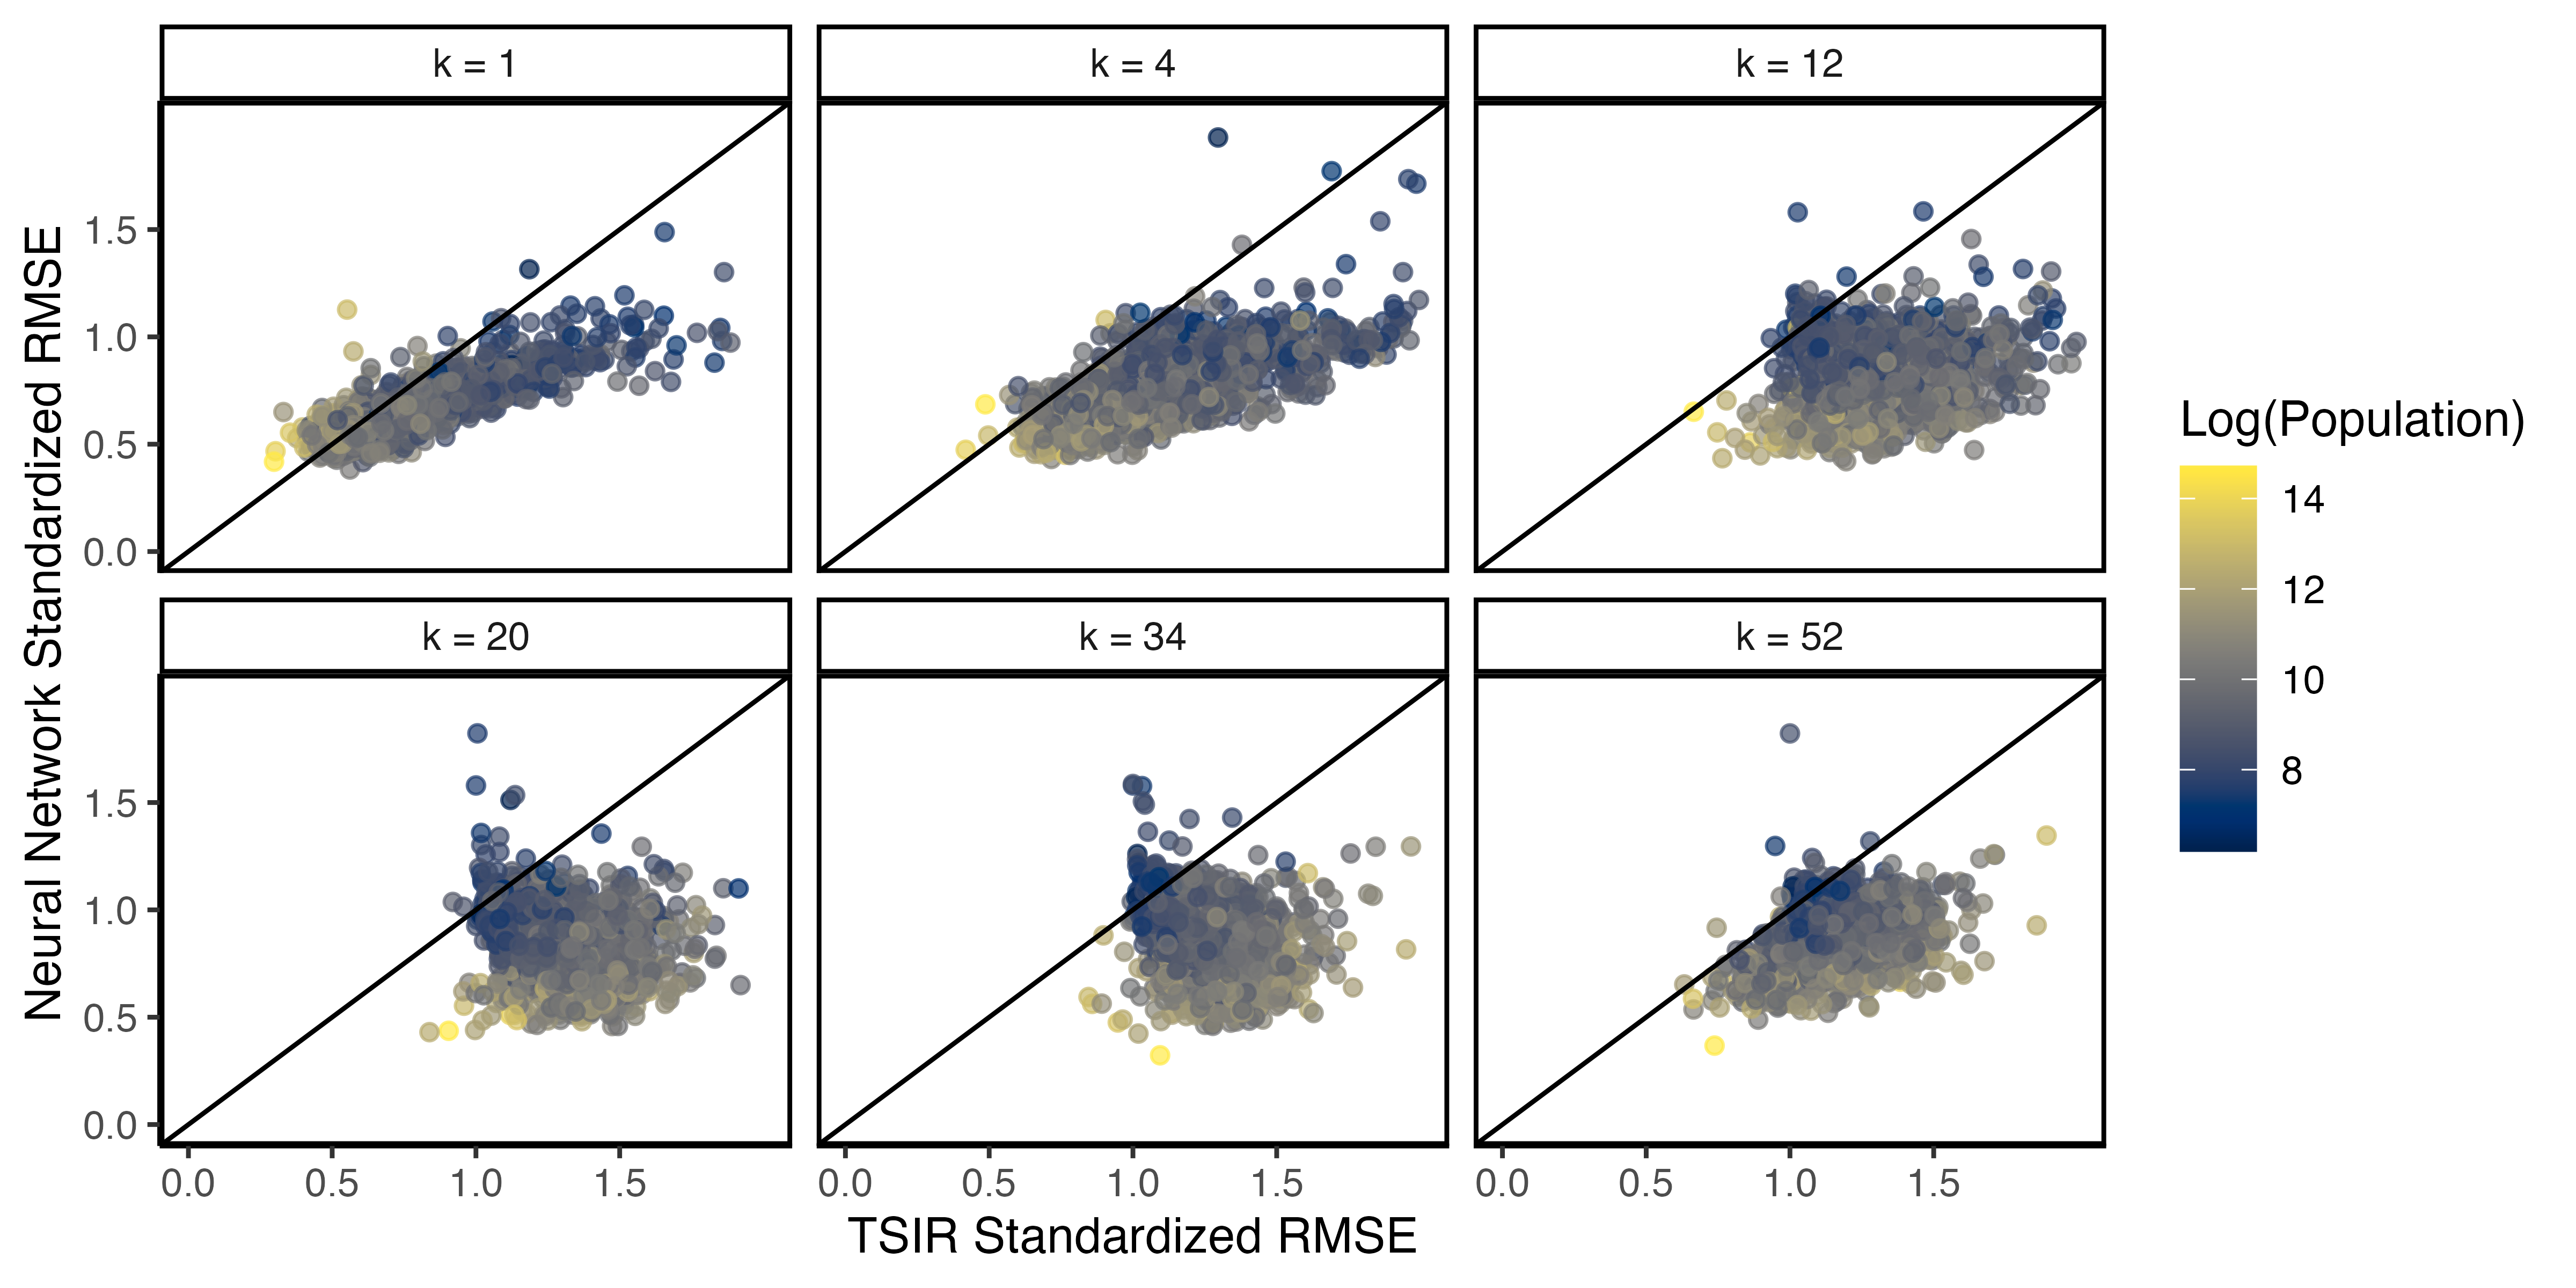
\includegraphics[width=1\linewidth]{figures/rmse_compare_nn_tsir_standardize_k_facet.png}
            \vspace{-2em}
             \label{fig:rmse}
        \end{tikzfigure}
    }

    \column{0.5}
    \block{Performance}{
        \begin{tikzfigure}[Within-city neural network prediction correlation with true cases over TSIR prediction correlation with true cases, colored by log(population), facetted by $k$-step ahead forecast.]
            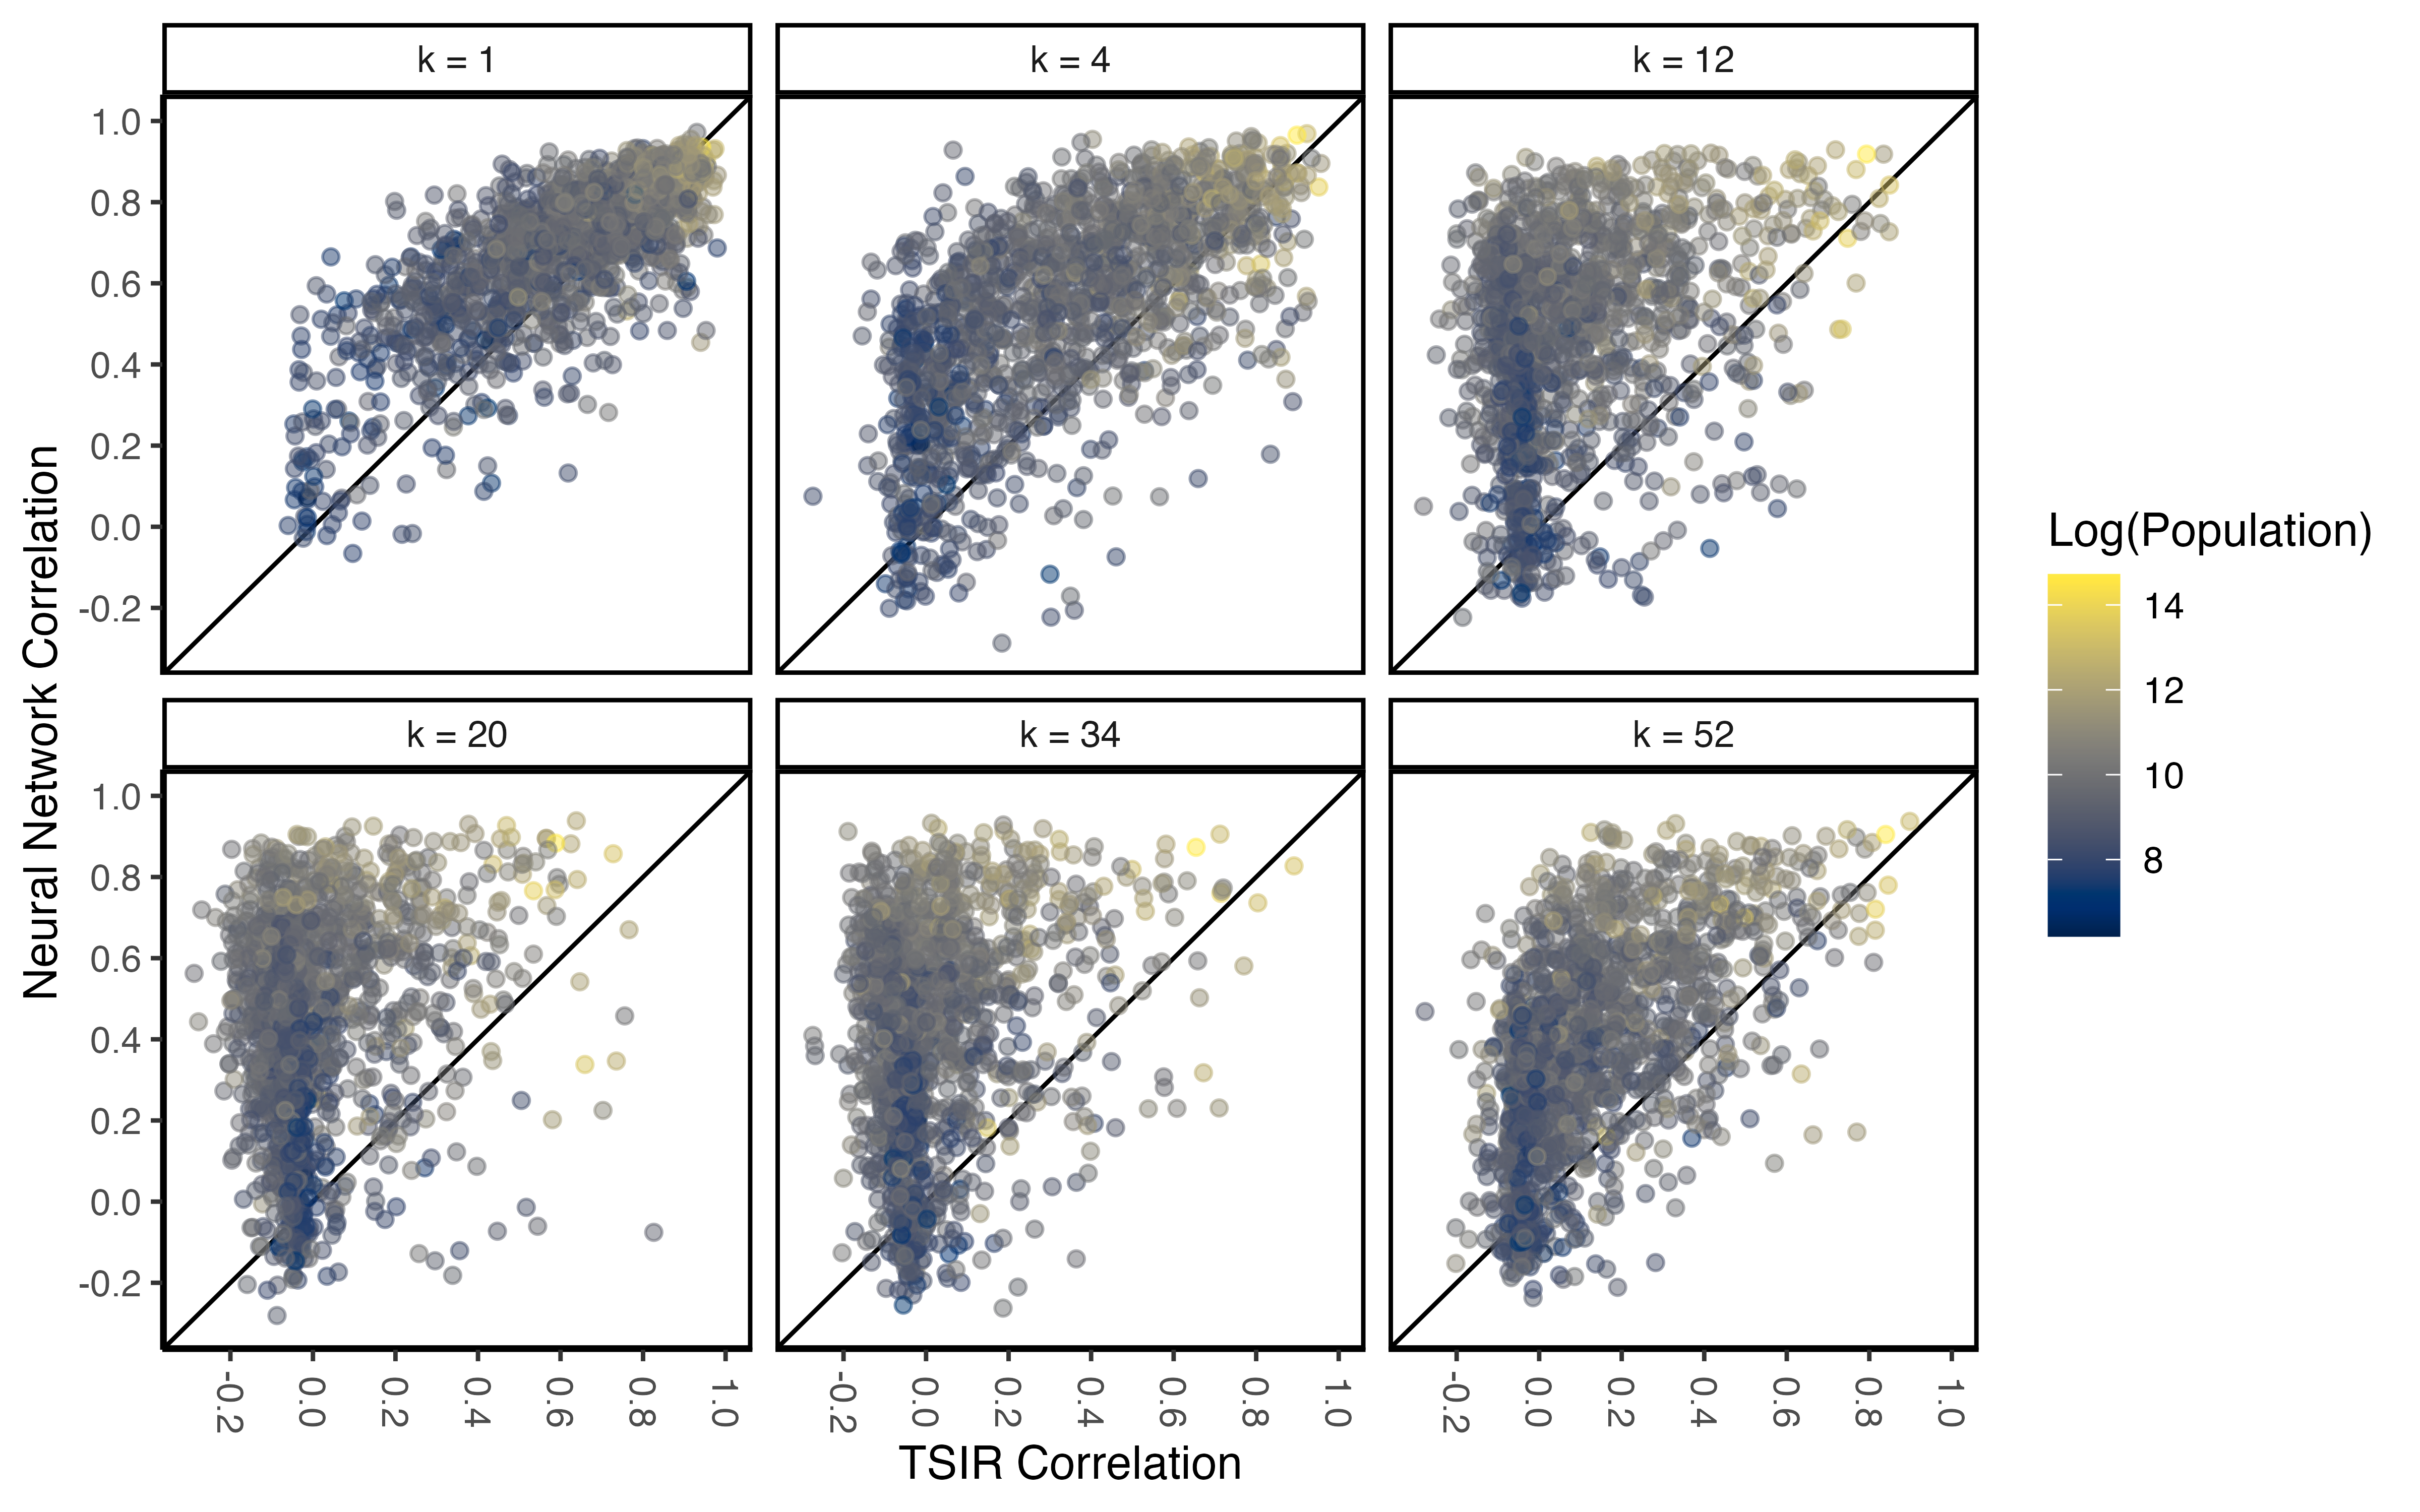
\includegraphics[width=1\linewidth]{figures/cor_nn_tsir_k_facet.png}
            \vspace{-2em}
             \label{fig:cor}
        \end{tikzfigure}
    }

    \block{Feature Importance}{
  \begin{minipage}{0.6\linewidth}
        \begin{tikzfigure}[Mean Absolute SHAP values by feature group.]
            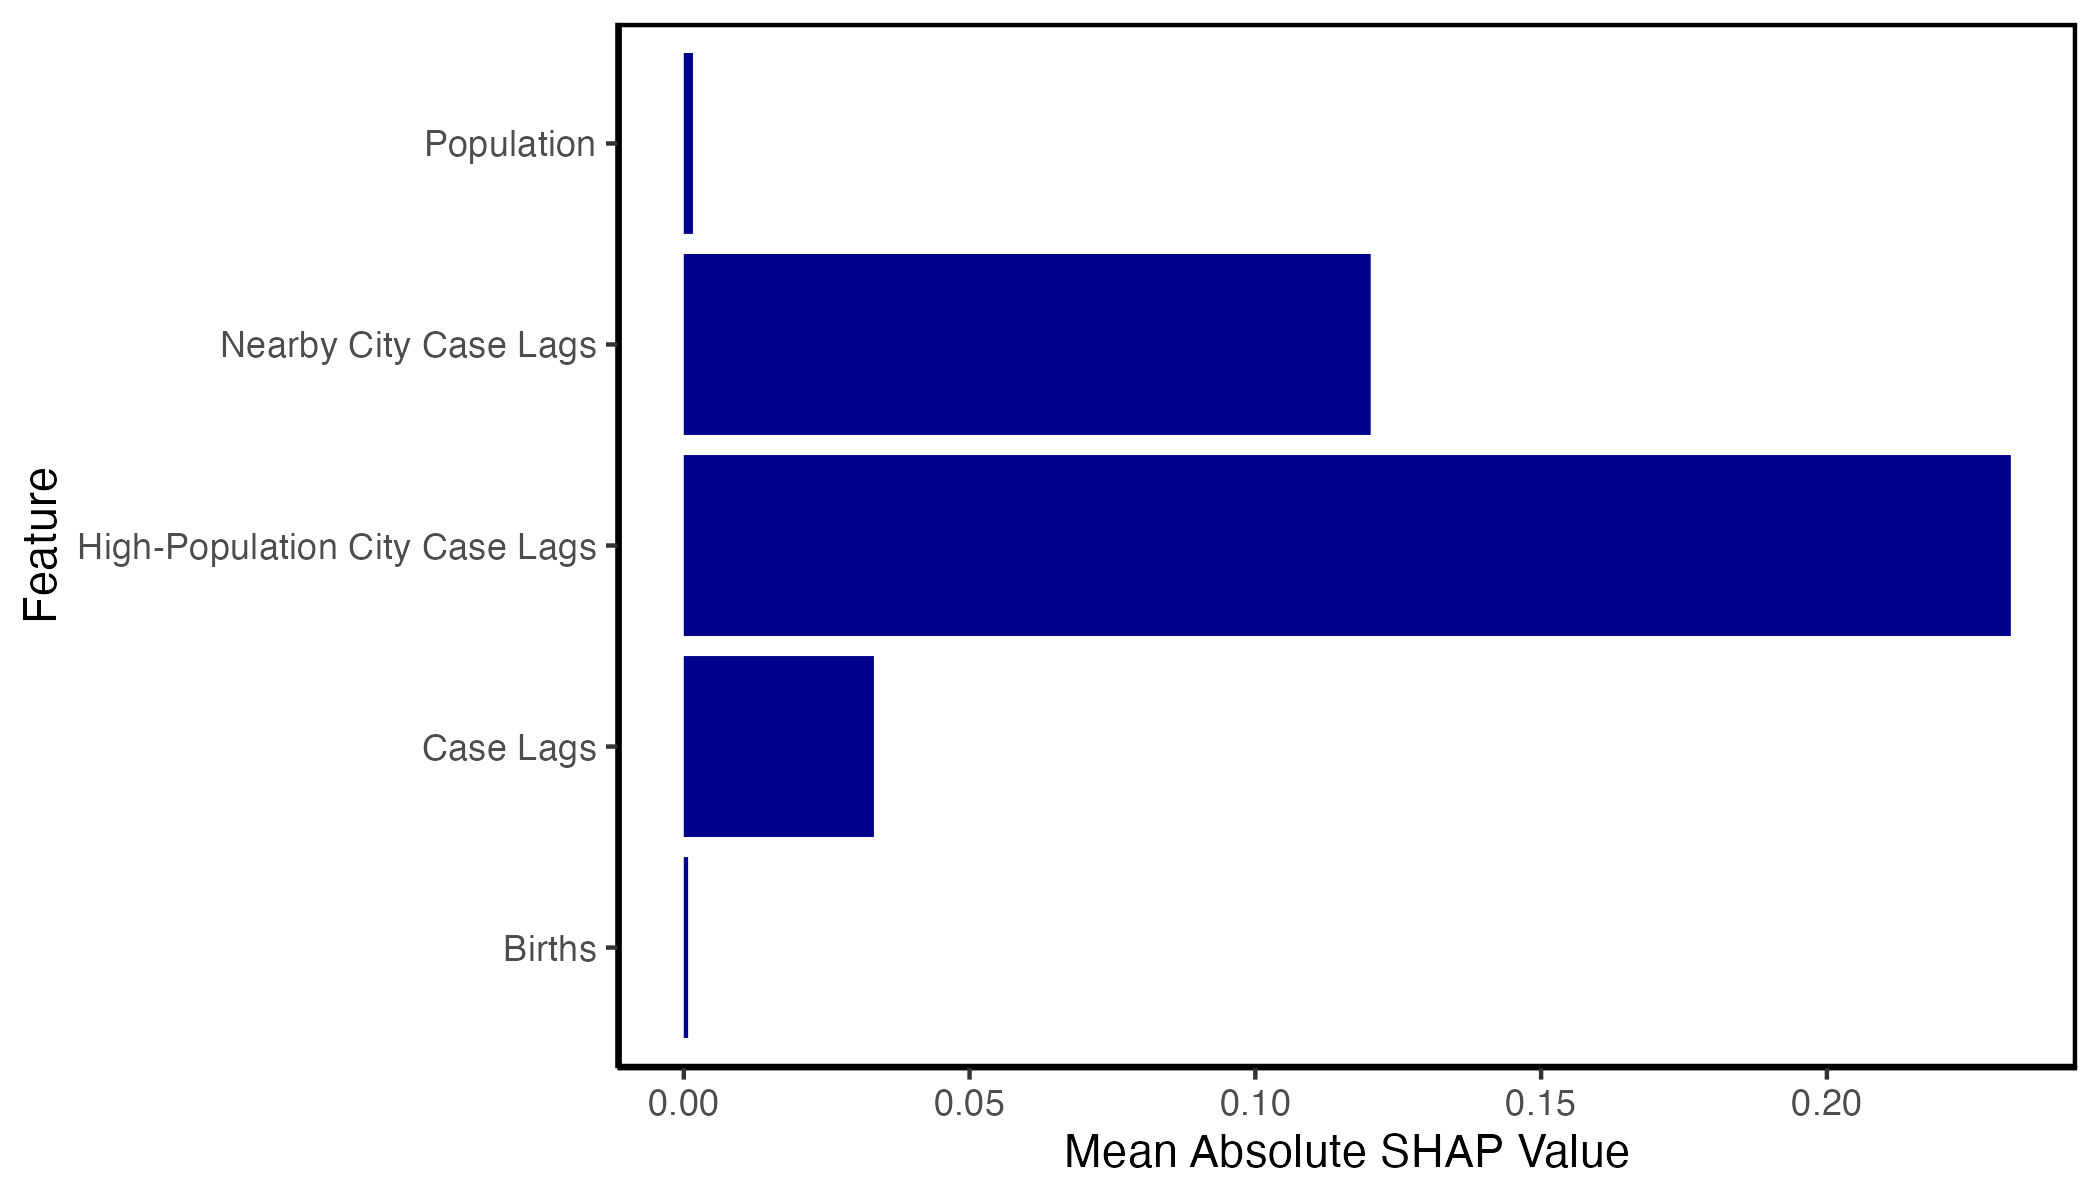
\includegraphics[width=0.7\linewidth]{figures/svs_abs_barplot.png}
            \vspace{-0.5em}
             \label{fig:svsbar}
        \end{tikzfigure}
            \vspace{1em}
  \end{minipage}
  \hfill
        \begin{minipage}{0.4\linewidth}
        We use the SHAP (SHapley Additive exPlanations) method \cite{lundberg2017unified} to assess feature importance.
        SHAP values are calculated by selected random permutations of feature groups, calculating the change in model output as each feature group is added back to a baseline value, and finally averaging across all permutations. 
        \end{minipage}%

        We choose to group features by lag type, e.g. all lagged nearest-city cases are grouped and permuted together.
        The mean absolute SHAP value for each feature group suggests that the most important features are the lagged case counts of high-population cities, followed by the lagged case counts of nearby cities/towns, and then the lagged case counts of the target city (Figure~\ref{fig:svsbar}).
        \vspace{2em}
    }


    \block{Gravity Dynamics}{


        Previous work has demonstrated the presence of gravity dynamics in measles outbreaks, where outbreaks in low population cities/towns are driven by outbreaks in nearby high population cities \cite{xia2004measles}.
        To assess if the neural network is learning high/low population epidemic coupling, we first calculate the relative absolute SHAP value for each feature group at each observation. 
        We then calculate the within-city mean value of the relative absolute SHAP values.
        This provides a measure of the relative importance of each feature group for each city.
        Plotting these against the log of the population of the target city, we see that the lagged case counts of high population cities are relatively more important for low population cities/towns, which suggests that our neural-network is able to reveal gravity-like core-satellite dynamics \cite{lau2020competing} present in the endemic measles spatio-temporal dynamics (Figure~\ref{fig:svsoverpop}).
        \begin{tikzfigure}[With-city mean relative absolute SHAP values over log(population) for each feature group, with LOESS fits.]
            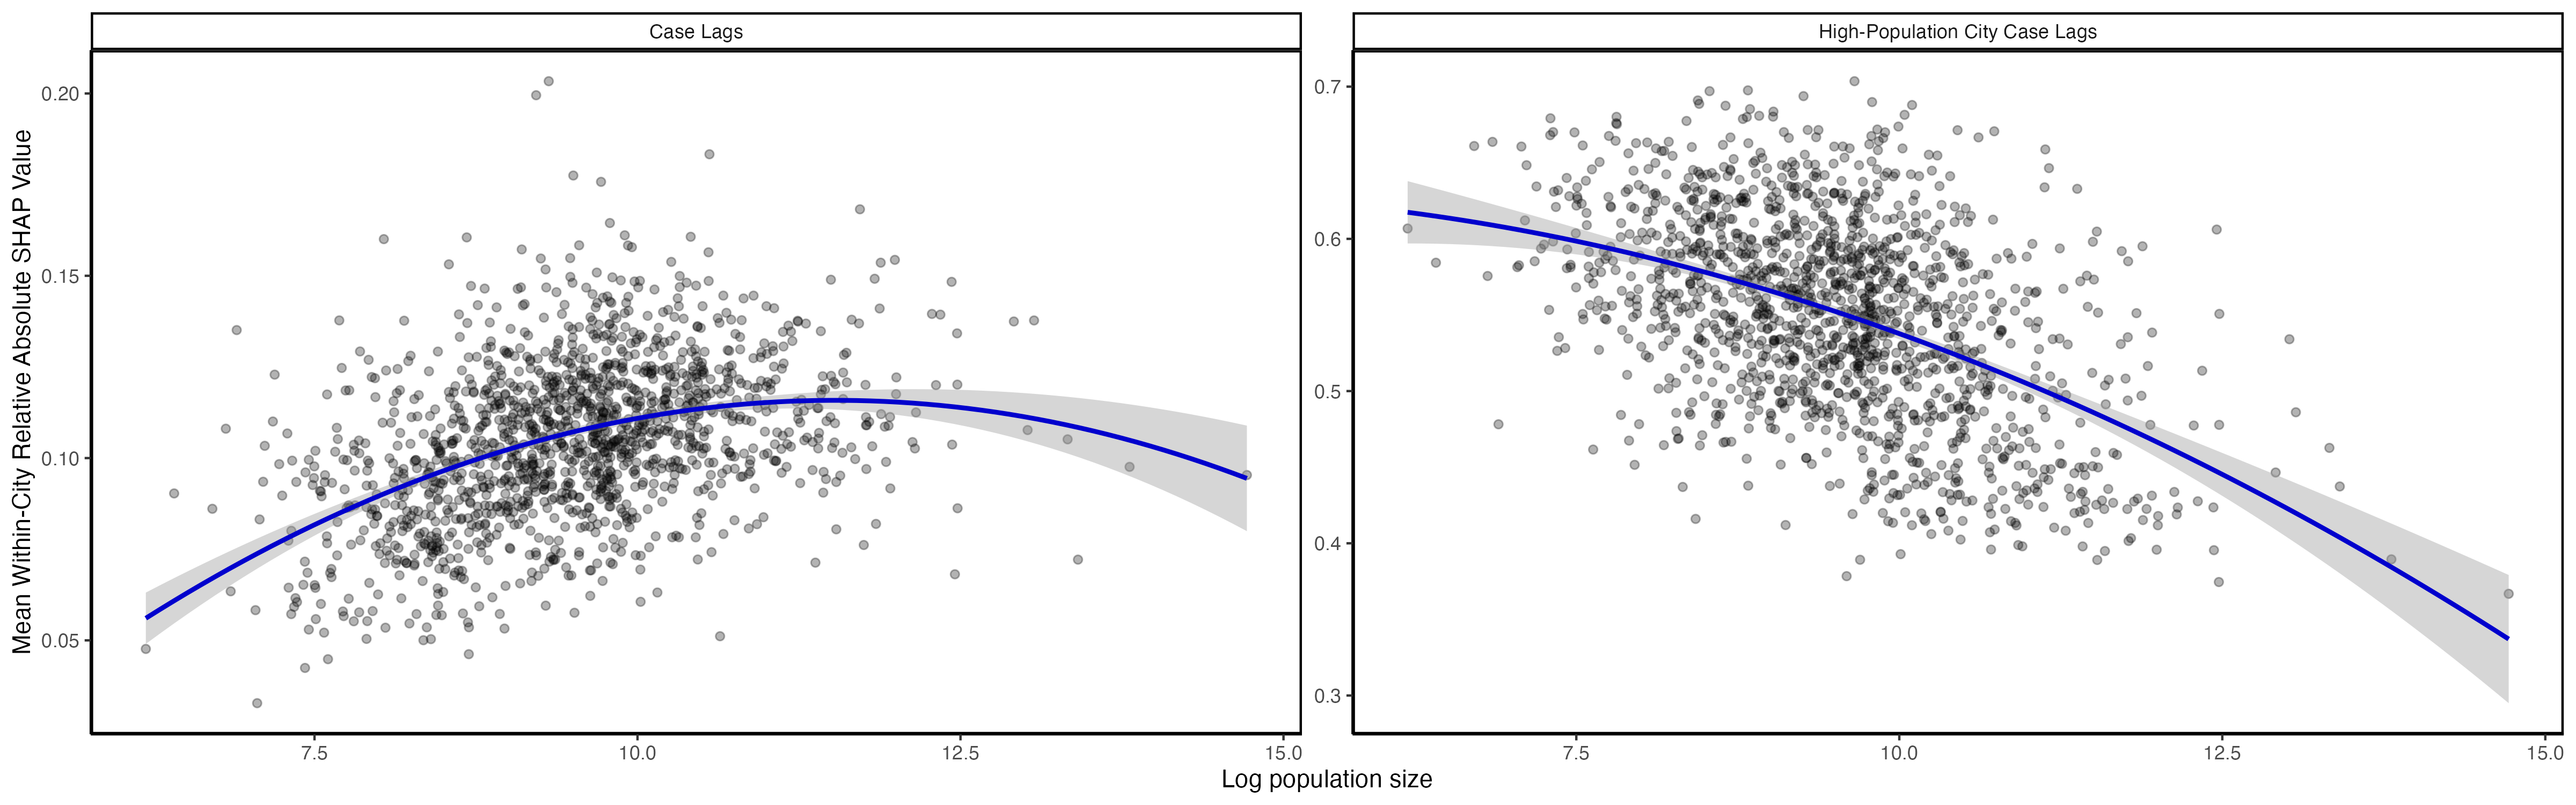
\includegraphics[width=0.9\linewidth]{figures/svs_mean_relwithinobs_abs_bycity_byvar.png}
            \vspace{-0.5em}
             \label{fig:svsoverpop}
        \end{tikzfigure}
        \vspace{2em}


     }

    \block{Future Directions}{
        \vspace{-1em}
        \begin{itemize}
            \item Extend analyses to more chaotic post-vaccination period.
            \item Explore joint approaches combining mechanistic models with neural networks, such as Physics-Informed Neural Networks (PINNs) and Neural-ODEs. 
        \end{itemize}
    }
    
    \block{Acknowledgements \& References}{
        This work is supported by the Dean’s Pilot and Innovation Awards provided by the Dean’s office at Rollins School of Public Health at Emory University. 
    \vspace{1em}
        \printbibliography[heading=none]
        
    }
\end{columns}
\end{document}
